\documentclass{article}

% Language setting
% Replace `english' with e.g. `spanish' to change the document language
\usepackage[portuguese]{babel}

% Set page size and margins
% Replace `letterpaper' with `a4paper' for UK/EU standard size
\usepackage[letterpaper,top=2cm,bottom=2cm,left=3cm,right=3cm,marginparwidth=1.75cm]{geometry}

% Useful packages
\usepackage{amsmath}
\usepackage{graphicx}
\usepackage[colorlinks=true, allcolors=blue]{hyperref}

\title{Exercício Programa 01 - Cálculo do Valor de \pi}
\author{Alexandre Barsam Junqueira}

\begin{document}
\maketitle

\begin{abstract}
Esse relatório busca desenvolver estimativas para o valor de $\pi$ por meio de Simulações de Monte Carlo, isto é: (i) gerar pontos uniformemente distribuídos $x_{i}\in[−1,1]^{2}$, $i\in\{1,…,n\}$; (ii) definir a proporção de pontos cuja distância do centro é menor que 1; (iii) estimar $\pi$. Além disso, busca-se entender um valor de $n$ ideal para um $erro \leq 0.05\%$.
\end{abstract}

\section{Introdução ao Método de Monte Carlo}

\subsection{Algoritmo e Utilização}

Criado por Stanislaw Ulam e John Von Neumann, o Método de Monte Carlo ou Simulação de Monte Carlo é um tipo de algoritmo computacional que utiliza amostragens aleatórias repetidas vezes para obter a probabilidade de um grupo de resultados ocorrer. O método é utilizado, principalmente, como forma de obter aproximações numéricas de funções complexas em que não é viável, ou é mesmo impossível, obter uma solução analítica ou determinística. Dessa forma, consegue-se atuar sobre problemas de otimização e integração numérica, por exemplo.

Na maioria dos casos, as simulações tendem a seguir um padrão:

\begin{enumerate}
    \item Definir um domínio de possíveis entradas;
    \item Gerar entradas randomicamente por meio de uma distribuição probabilística sobre o domínio;
    \item Obter resultados para cada entrada;
    \item Juntar os resultados.
\end{enumerate}

Desse modo, o Método de Monte Carlo é uma ferramenta extremamente poderosa para o entendimento de situações complexas e para aproximações. No entanto, traz consigo problemas relacionados a custo computacional, precisão e dimensionalidade.

\subsection{Intervalo de Confiança ($IC$) e Margem de Erro ($e$) para Proporções Populacionais}

Por se tratar de um modelo probabilístico, não basta somente conduzir uma simulação e obter o resultado, é preciso entender a relevância estatística daquele resultado. Por isso, cabe observar o intervalo de confiança e a margem de erro do modelo.

Quando se deseja entender a proporção $p$ de uma população de tamanho $m$ que possui determinada característica x, $p = \frac{n_x}{m}$. No entanto, muitas vezes é imprático abordar toda a população, sendo preferível observar amostras aleatórias de tamanho $n$. Dessa forma, pode-se utilizar a proporção amostral $p_a$ para estimar $p$.

Com o $n$ grande, obtem-se uma aproximação de uma curva normal: $p_a \approx N(p, \frac{p\sart{1-p}}{n})$. Assim, é possível obter um Intervalo de Confiança com coeficiente de confiança $\gamma$:
$$IC_p = \left[p_a - z_\gamma \cdot \sqrt{\frac{p_a (1 - p_a)}{n}}, p_a + z_\gamma \cdot \sqrt{\frac{p_a (1 - p_a)}{n}}\right]$$

Definindo-se a margem de erro como metade do tamanho do intervalo de confiança, tem-se que: $$e = z_\gamma \cdot \sqrt{\frac{p_a (1 - p_a)}{n}}$$ $$n = \left(\frac{z_\gamma}{e}\right)^{2}  p_a \cdot (1 - p_a)$$

Com isso, consegue-se determinar um tamanho da amostra $n$ para o qual é possível obter uma estimativa para $p$ com erro $e$ e confiança de $\gamma$.

Como $\pi = 4p$, sendo $p = \frac{n_{dentro}}{n_{total}}$, tem-se que $\pi_a = 4p$ e $\sigma_{\pi_m} = 4\sigma_{p_m}$. Assim:
$$IC_\pi = \left[\pi_a - 4z \cdot \sqrt{\frac{p_a \cdot (1 - p_a)}{n}}, \pi_a + 4z \cdot \sqrt{\frac{p_a \cdot (1 - p_a)}{n}}\right]$$

Portanto, analogamente ao processo anterior, tem-se que:
$$n_\pi = 16\cdot\left(\frac{z}{e}\right)^{2} \cdot p_a \cdot (1 - p_a)$$

Similarmente, no pior dos casos:
$$n_\pi=4\cdot\left(\frac{z}{e}\right)^{2}$$

\section{Cálculo do Valor de $\pi$ com o Método de Monte Carlo}

\subsection{Algoritmo para a Estimativa}
A Simulação de Monte Carlo consegue obter uma aproximação do valor de $\pi$. Mais precisamente, isso pode ser alcançando pelas seguintes etapas - exemplificado de maneira visual na Figura 1:

\begin{enumerate}
    \item Determinar um quadrado no plano cartesiano por $x\in[-1, 1]$ e por $y\in[-1, 1]$;
    \item Dispersar uniformemente um número de $n$ de pontos dentro do quadrado;
    \item Verificar a quantidade $n_d$ de pontos cuja distância da origem é menor que 1, isto é, que estão dentro do círculo unitário;
    \item A razão $\frac{n_d}{n}$ aproxima-se da razão da área da circunferência pela área do quadrado. Logo, $\frac{n_d}{n} \approx \frac{\pi}{4}$;
    \item Com isso, estima-se $\pi \approx \frac{4 \cdot n_d}{n}$.
\end{enumerate}

\begin{figure}[h]
\centering
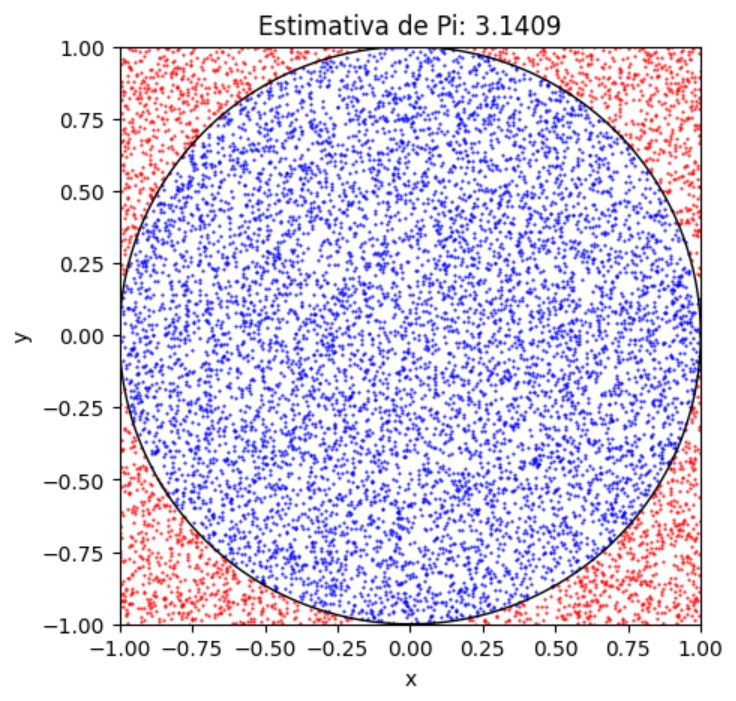
\includegraphics[width=0.50\linewidth]{Figura 1.jpg}
\caption{\label{fig:Figura 1}Exemplificação visual do Método de Monte Carlo para o cálculo de $\pi$.}
\end{figure}

\subsection{Intervalo de Confiança  e Margem de Erro}

Essa Simulação de Monte Carlo para o cálculo do valor de $\pi$ é um problema de proporção populacional: de todos os pontos contidos dentro do quadrado, qual fração deles está dentro do círculo unitário. Sendo impossível computar todos os pontos nessa área, pode-se pegar uma amostra aleatória para estimar $p$ por meio de $p_a$.

Dessa maneira, para definir o tamanho da amostra, precisa-se estabelecer o erro, o grau de confiança e uma proporção amostral. Assumindo $e = 0,05\%$ e $\gamma = 95\%$ (e, logo, $z_\gamma \approx 1,96$), falta definir $p_a$.

Conhecendo o valor de $\pi$, sabe-se que $p = \frac{\pi}{4}$. Não obstante, tomando esse valor como desconhecido, pode-se obter um valor de $p_a$ satisfatório conduzindo diversas amostragens aleatórias e utilizando a média dos valores de $\pi$ encontrados.

A Figura 2 demonstra a distribuição do valor de $\pi$ encontrado em $10^6$ amostragens aleatórias com $n = 10^3$. A média desses valores foi de $\mu \approx 3.1416$ com erro padrão $\sigma_m \approx 0,00013$.

\begin{figure}[h]
\centering
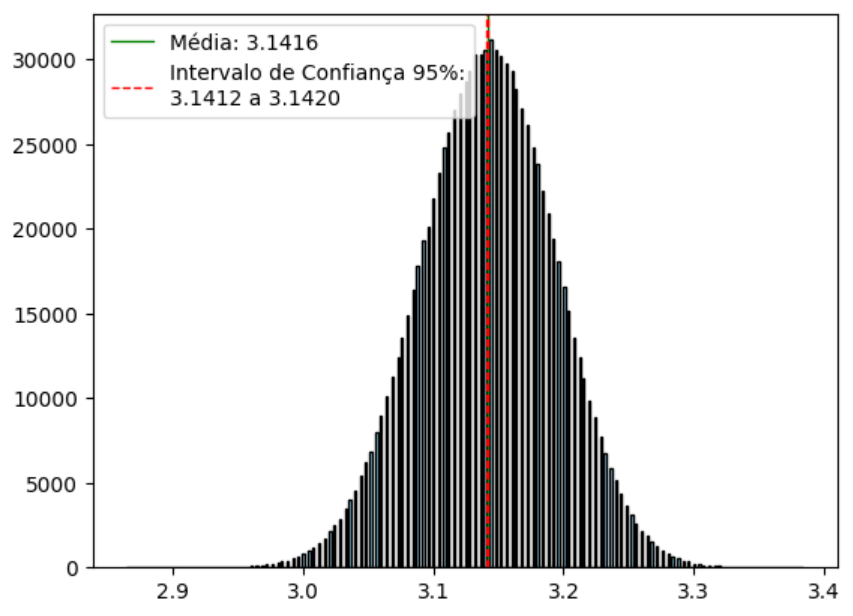
\includegraphics[width=0.60\linewidth]{Figura 2.png}
\caption{\label{fig:Figura 2}Distribuição das estimativas para $\pi$ nas amostragens.}
\end{figure}

Com isso, utilizando $p_a = \frac{\mu}{4}$, obtém-se que
$$n_\pi = 41.458.544$$

Outra opção quando se desconhece uma estimativa para $p$ é simplesmente supor o caso em que $n$ seja o maior possível, isto é, $p = 0,5$, resultando em:
$$n_\pi = 61.465.600$$

\subsection{Análise de Convergência}

Por fim, uma última maneira de compreender um valor propício para o tamanho da amostra $n$ é observar graficamente a convergência das estimativas para o valor real. Como pode ser visto nas imagens a seguir, as estimativas de $\pi$ apresentam um erro consistentemente abaixo de $0,05\%$ a partir de $3 \cdot 10^6$. No entanto, isso foi feito com poucas repetições, tornando o resultado obtido por intervalo de confiança e margem de erro uma melhor recomendação para $n$.

\begin{figure}[h]
    \begin{minipage}[!]{0.5\linewidth}
    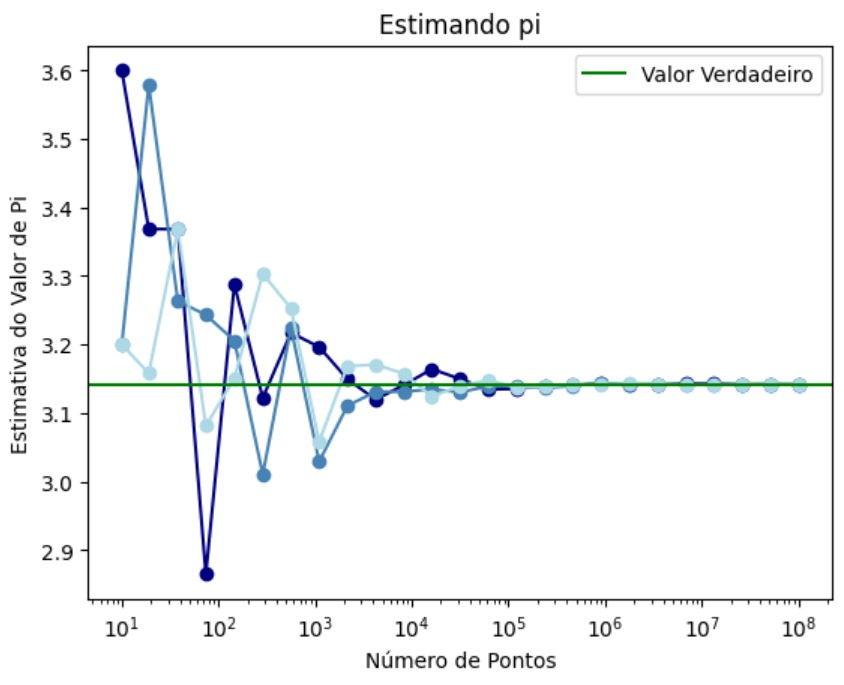
\includegraphics[width=1\linewidth]{Figura 3-1.jpg}
    \end{minipage}
    \begin{minipage}[!]{0.5\linewidth}
    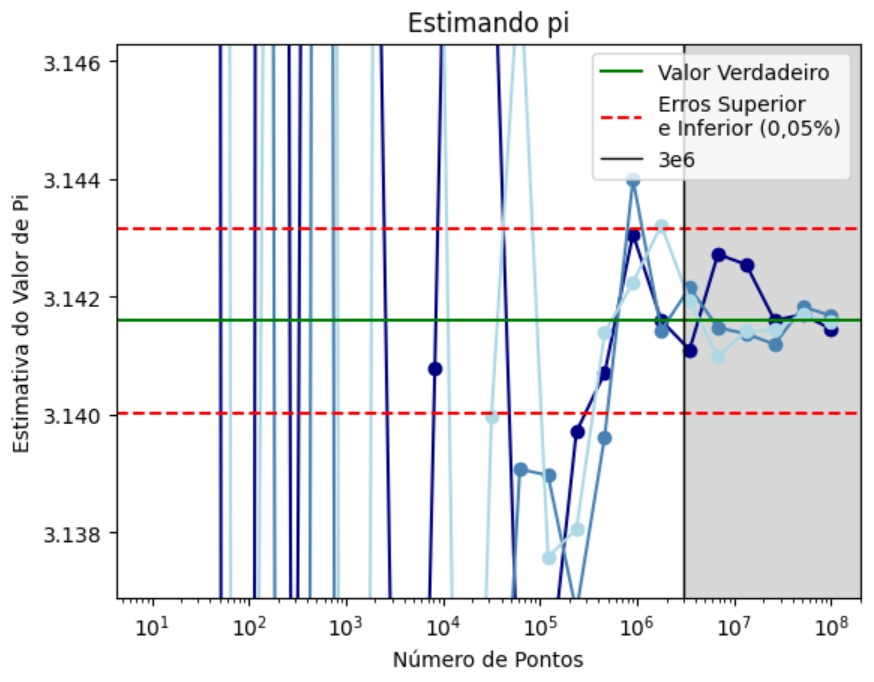
\includegraphics[width=1\linewidth]{Figura 3-2.jpg}
    \end{minipage}
    \caption{\label{fig:Figura 3}Simulações de Convergência com o aumento de $n$.}
\end{figure}

\begin{figure}[h]
\centering
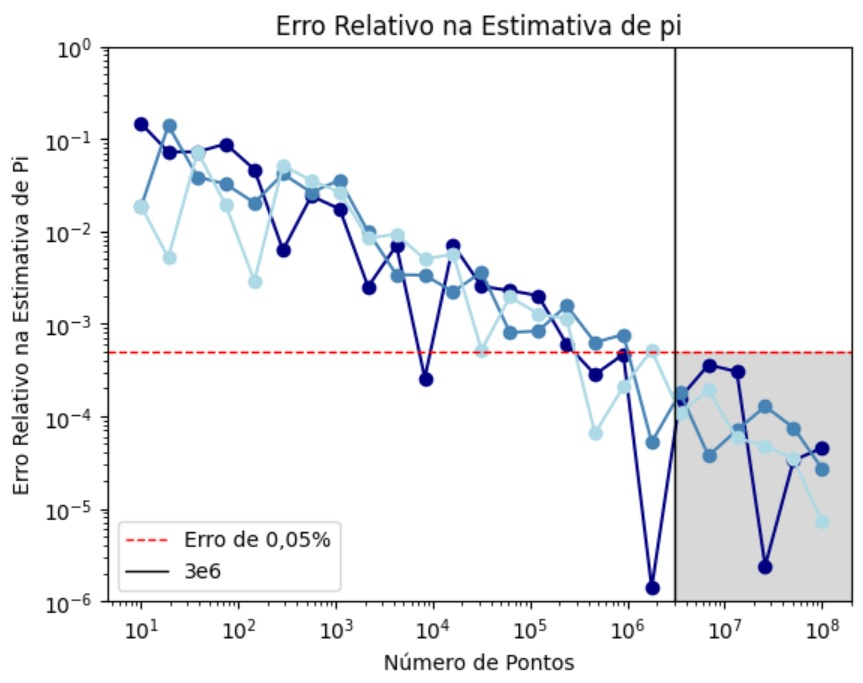
\includegraphics[width=0.60\linewidth]{Figura 4.jpg}
\caption{\label{fig:Figura 4}Análise do erro relativo das simulações conduzidas e sua evolução.}
\end{figure}.

\end{document}